% This chapter is based on:
%   Rian Touchent et al.
%   The CLM Detour: Computational Hysteresis Improves
%   Encoder Continued Pretraining.
%   COLM, 2026.

\section{Introduction}

\begin{reviewread}
Much of the recent progress in language modeling has happened on the decoder side. Large decoders brought longer context windows, faster attention implementations, cleaner data pipelines, and the causal language modeling objective at scale. Continued pretraining these models on biomedical text, however, is no longer an obvious win. The biomedical literature is already present in many web-scale corpora, and narrow continued pretraining can damage the instruction-following and general reasoning abilities that make these models useful.
\end{reviewread}

\begin{reviewread}
For this thesis, the useful lesson is that some of the machinery developed for decoders can be reused for encoders. We take a modern encoder architecture, train it on a biomedical corpus curated with the same attention to data quality that improved recent decoder corpora, and borrow the causal objective for the main pretraining phase. The model is then converted back to masked language modeling so that it remains an encoder at fine-tuning time.
\end{reviewread}

\begin{reviewread}
In this chapter, we introduce a two-phase pretraining strategy for ModernCamemBERT-bio: first, continual pretraining with a causal language modeling objective, then a short ``decay'' phase that converts the model back to masked language modeling. The resulting encoder outperforms the standard MLM-only approach by +2.9 $F_1$ on average across 8 French biomedical tasks (Base) and +1.5 $F_1$ (Large), winning on all 8. The effect transfers to English at three scales, with gains of +0.3 to +0.8 $F_1$ depending on model size.
\end{reviewread}

\begin{reviewread}
The CLM phase leaves a lasting imprint on low transformer layers. CKA analysis shows that layers 0--7 diverge 5--44$\times$ more between CLM and MLM models than seed noise alone, and this divergence persists through extended MLM decay. Freeze interventions establish a double dissociation: freezing low layers during CLM eliminates the downstream benefit; freezing mid layers preserves it. The advantage cannot be localized after training: transplanting layer groups from the CLM model into the MLM model recovers at most 35\% of the gap, because the benefit depends on how the layers co-adapt during training rather than on any single group.
\end{reviewread}


\section{Motivation}

\subsection{Lessons from Decoder Pretraining}
\label{sec:decoder-cpt-stops}

Recent biomedical language models often start from a large generalist decoder and continue its pretraining on biomedical data. This is the recipe behind models such as BioMistral and Meditron. It is an important change in the field, but its lesson for this thesis is mixed. Decoder continued pretraining has become expensive and less reliable as general models have grown. At the same time, the decoder literature has improved the tools around pretraining, including longer-context architectures, dense causal objectives, and stronger corpus filtering. We keep those tools, but apply them to encoders.

The large models have, for the most part, already read the biomedical literature. PubMed abstracts and PubMed Central are part of the web corpora these models are pretrained on, so continued pretraining largely shows them text they have already seen. The measured effect is often negative. \citet{dorfner2024biomedical} compare biomedical models against the general models they were built from and find the biomedical versions usually worse, with OpenBioLLM-8B scoring 30.0\% on clinical case questions against 64.3\% for Llama-3-8B. \citet{labrak-etal-2024-biomistral} report the same for BioMistral, whose accuracy on medical multiple-choice questions falls well below the Mistral model it continues and is recovered only by merging the two back together.

Continued pretraining also damages what made the generalist useful. A large model earns its value by following instructions and reasoning across domains, and training it on a narrow corpus erodes exactly those abilities, a forgetting of skills rather than of facts. \citet{jindal_balancing_2024} measure a drop of about ten points on an instruction-following benchmark after only a billion tokens of continued pretraining, even as a knowledge proxy improves; replay and merging recover part of the loss but are unreliable at scale. And the price is steep: Meditron-70B took on the order of forty thousand A100-hours of continued pretraining for an average gain of under two points on biomedical benchmarks~\citep{chen2023meditron}. These are not early-days artefacts. On a new French health corpus, \citet{mannion_biomedical_2026} find that domain-adaptive pretraining of decoders helps only the smallest models and that its benefit has vanished by the eight-billion-parameter scale.

For clinical information extraction, the comparison runs the other way. A small encoder fine-tuned on the task still matches or beats a much larger decoder at a fraction of the compute. \citet{obeidat_do_2025} report that encoders trail eight-billion-parameter models by only a few points on biomedical named entity recognition while running tens to hundreds of times faster, and win outright on several datasets. \citet{lehman_we_2023} had already shown that a small in-domain clinical model beats in-context learning with a far larger one, even under limited annotation. Deployment also favours encoders, since a clinical extractor has to run inside the hospital, on modest hardware, on data that cannot be sent to an outside provider.

The useful lesson is to separate decoder continued pretraining from the decoder pretraining recipe. Recent decoder models have improved the recipe itself. OLMo 2, for example, combines autoregressive decoder training with stability fixes, modern architecture choices, and a curated late-stage data mixture~\citep{olmo2025furious}. These changes remain useful when the final model is an encoder because they concern how much signal each token provides, how training stays stable, and how the corpus is selected.

This makes the causal objective worth revisiting for encoders. \citet{gisserot2025clm} control for scale and data by training matched models from 210M to 1B parameters. They find that MLM remains stronger on average for representation tasks, but that CLM is more data-efficient and gives more stable fine-tuning. Their best fixed-budget recipe trains first with CLM and then returns to MLM. The rest of the chapter tests the same direction in a biomedical continued-pretraining setting. We start from pretrained encoders, adapt them to biomedical text, and ask whether a temporary CLM phase leaves a useful trace after returning to MLM.

One reason to expect a gain is that MLM makes poor use of its tokens at training time. With 15\% masking, the model sees a full sequence but only receives a training signal on about 15 of every 100 positions, since the loss is computed on the masked positions alone. The remaining tokens are read as context and never predicted. CLM computes a loss at every position, so the same sequence yields several times more predictions for the same forward and backward pass. For a fixed token budget, this is a large difference in how much supervision the model extracts from the corpus.

\subsection{Architecture and Objective}

\begin{reviewread}
CamemBERT-bio (\Cref{chap:encoders}) demonstrated that continual pretraining works for biomedical encoders. However, it used the original CamemBERT architecture: 512-token context, absolute position embeddings, no Flash Attention. Clinical documents are often longer than 512 tokens, and the architecture has not kept pace with recent advances.
\end{reviewread}

\begin{reviewread}
ModernBERT~\citep{modernbert} addresses these limitations with Flash Attention, RoPE position embeddings, alternating local/global attention, and an 8,192-token context window. For biomedical adaptation, we start from ModernCamemBERT (French) and ModernBERT (English), in both Base (150M) and Large (350M) sizes.
\end{reviewread}

\begin{reviewread}
The standard approach would be to continue MLM pretraining on biomedical data, as we did for CamemBERT-bio. But MLM has a structural limitation: only 15\% of tokens are masked and receive gradient signal at each step. Causal language modeling avoids this: every token predicts the next, so every position contributes to the loss. The idea is to use CLM for the compute-intensive pretraining phase, and switch back to MLM only at the end, to recover bidirectional attention. The key question is whether this switch erases the benefits of CLM or preserves them.
\end{reviewread}

\paragraph{Related approaches.} Recent work has started to compare objective switching under controlled conditions. \citet{ettin2025} train matched encoder/decoder pairs (up to 1B parameters, 1.7T tokens) and show that continued pretraining on the reverse objective does not bridge the encoder-decoder performance gap. AntLM~\citep{antlm2024} alternates between CLM and MLM epochs at small scale (10M words). Our approach differs in three ways: we study the round-trip MLM$\to$CLM$\to$MLM with continued pretraining, we focus on the lasting effect of the CLM phase after returning to MLM, and we provide causal evidence via freeze interventions of where the benefit comes from. As \citet{gisserot2025clm} note, understanding how training objectives transfer to downstream tasks ``remains largely unexplored.''


\section{Method}
\label{sec:clm-detour}

\subsection{The CLM Detour}

\begin{reviewread}
Our approach consists of two phases, illustrated in \Cref{fig:clm-pipeline}.
\end{reviewread}

\begin{figure}[t]
\centering
\begin{tikzpicture}[node distance=1.8cm, >=Stealth, scale=0.85, transform shape,
  box/.style={rectangle, rounded corners=3pt, draw=ThesisNeutral, minimum height=0.9cm, minimum width=2.4cm, align=center, font=\small\sffamily}
]
  \node[box, fill=ThesisPrimary!20] (base) {MLM encoder\\(ModernBERT)};
  \node[box, fill=ThesisTertiary!30, right=of base] (clm) {CLM phase\\(10--50B tokens)};
  \node[box, fill=ThesisSecondary!30, right=of clm] (decay) {MLM decay\\(10\% of Phase 1)};
  \node[box, fill=ThesisPrimary!30, right=of decay] (out) {ModernCamem-\\BERT-bio};

  \draw[->, thick, ThesisNeutral] (base) -- (clm) node[midway, above, font=\tiny\sffamily] {causal mask};
  \draw[->, thick, ThesisNeutral] (clm) -- (decay) node[midway, above, font=\tiny\sffamily] {bidir.\ mask};
  \draw[->, thick, ThesisNeutral] (decay) -- (out);
\end{tikzpicture}
\caption{\textbf{The CLM detour pipeline.} Starting from a pretrained MLM encoder, we continue pretraining with a causal objective (Phase~1), then decay back to MLM (Phase~2). The model does not return to an MLM-like state.}
\label{fig:clm-pipeline}
\end{figure}

\paragraph{Phase 1: CLM pretraining.} Starting from a pretrained ModernBERT encoder, we replace the bidirectional attention mask with a causal mask and train with next-token prediction. The model architecture is unchanged: only the attention mask and loss computation differ. This forces the model to compress information into each token representation, since it cannot look ahead.

\paragraph{Phase 2: MLM decay.} After CLM pretraining, we restore bidirectional attention and train with MLM at 15\% masking for approximately 10\% of the Phase~1 budget. The optimizer state is kept between phases; only the learning rate scheduler resets. Phase~2 decays the learning rate from peak to 10\% of peak.

\paragraph{Controlled comparison.} The MLM baseline follows the same two-phase structure with 30\% masking in Phase~1 and 15\% in Phase~2, identical schedule and optimizer. Both trajectories use identical architecture, data, and total compute. We write $\Phi_{1,\text{CLM}}$ for a Phase~1 of causal training, $\Phi_{1,\text{MLM}30\%}$ for a Phase~1 of masked training at 30\% masking, and $\Phi_{2,\text{MLM}15\%}$ for the shared Phase~2 decay at 15\% masking. Each operator takes a set of weights and a token budget, and returns the weights obtained after training on that budget:
\begin{align*}
\theta_A &= \Phi_{2,\text{MLM}15\%}(\Phi_{1,\text{CLM}}(\theta_0, n),\; 0.1n) && \text{(CLM detour)} \\
\theta_B &= \Phi_{2,\text{MLM}15\%}(\Phi_{1,\text{MLM}30\%}(\theta_0, n),\; 0.1n) && \text{(MLM baseline)}
\end{align*}
Here $\theta_0$ is the pretrained encoder we start from, $n$ is the Phase~1 budget, and $0.1n$ is the Phase~2 budget. Both trajectories therefore train on $1.1n$ tokens in total and share the same Phase~2.
\begin{reviewread}
The only difference is the Phase~1 objective. Any performance gap is attributable to the training objective alone.
\end{reviewread}

\subsection{Data}

\paragraph{French.} We compile 10B tokens (Base) or 25B tokens (Large) from four sources. The main source (7B tokens) is French biomedical literature (scientific articles, clinical guidelines, medical theses), where each paragraph is scored for educational value using Qwen3-235B and articles are upsampled based on their proportion of high-scoring paragraphs, following the Biomed-Enriched approach (\Cref{chap:quality}). The remaining sources are synthetic medical QA from French coding systems (2B), clinical cases from the European Clinical Case Corpus (E3C, 400M), and drug package inserts from the European Medicines Agency (600M).

\paragraph{English.} For the 50B scale, we mix three components: 60\% biomedical literature from Biomed-Enriched (PMC Open Access articles filtered by educational value $\geq 3.0$), 20\% medical instruction-following datasets (MedS-Ins~\citep{wu2025medsins}, ReasonMed~\citep{sun2025reasonmed}, MediFlow~\citep{corbeil2025mediflow}, UltraMedical~\citep{zhang2024ultramedical}, EHR-Ins-Reasoning~\citep{liao2025ehrr1}), and 20\% MIMIC-III discharge summaries and clinical notes. The smaller 10B variant uses Biomed-Enriched with clinical case paragraphs upsampled 100$\times$ and other clinical documents 10$\times$ (80\%), plus MediFlow medical instructions (20\%), without MIMIC.

\subsection{Training Details}

\begin{reviewread}
All runs use decoupled AdamW with peak lr $2 \times 10^{-4}$, $\beta_1 = 0.9$, $\beta_2 = 0.98$, weight decay $10^{-5}$, and a global batch size of 384 sequences ($\sim$3.1M tokens). Phase~1 uses linear warmup over 100M tokens then constant learning rate. Documents are packed into 8,192-token sequences with end-of-sequence tokens between documents. Training uses bf16 mixed precision on 4$\times$H100 GPUs.
\end{reviewread}

\subsection{Fine-tuning Protocol}

\paragraph{French tasks.} Single-label classification (DiaMED~\citep{drbenchmark2024}) and multilabel classification (MedDialog \citep{liu2024meddialog}, FrACCO \citep{pignat2024fracco}, CANTEMIST \citep{miranda2020cantemist}, DisTEMIST \citep{miranda2022distemist}) use a linear head on the CLS token, trained for 15 epochs with lr $= 2 \times 10^{-5}$, batch size 4, and 10\% warmup. The multilabel classification tasks use max sequence length 4096 with weighted BCEWithLogitsLoss; single-label classification uses 2048. NER tasks (EMEA and Medline, from QUAERO~\citep{neveol14quaero}) use a span-based architecture with BiLSTM, CRF, and biaffine scorer, trained for 4000 steps with lr $= 5 \times 10^{-5}$ for the encoder and $10^{-3}$ for the head, batch size 16, max length 1024. All tasks use AdamW with weight decay 0.01 and select the best checkpoint by validation $F_1$.

\paragraph{English tasks.} We follow the BioClinical-ModernBERT evaluation protocol~\citep{sounack2025bioclinicalmodernbert}: lr $= 5 \times 10^{-5}$, weight decay 0.01, batch size 16, 10 epochs for most tasks (20 for NER). All models are fine-tuned with the same hyperparameters per task.

\subsection{Evaluation}

\begin{reviewread}
We evaluate on 8 French and 11 English biomedical tasks (\Cref{tab:eval-tasks}), using 9 seeds for French and 5 for English. French baselines include ModernCamemBERT, DrBERT~\citep{labrak2023drbert}, CamemBERT-bio, and CamemBERT~\citep{martin-etal-2020-camembert}. English baselines include ModernBERT, PubMedBERT~\citep{gu_domain-specific_2022}, BioBERT~\citep{lee_biobert_2019}, and BioClinical-ModernBERT~\citep{sounack2025bioclinicalmodernbert}.
\end{reviewread}

\begin{table}[t]
\centering
\small
\begin{tabular}{llcc}
\toprule
\textbf{Task} & \textbf{Type} & \textbf{Lang} & \textbf{Max len.} \\
\midrule
\rowcolor{ThesisTableSep} \multicolumn{4}{c}{\rule{0pt}{9pt}\textbf{French}} \\[1pt]
DiaMED & Classification & FR & 2048 \\
MedDialog-FR & Multilabel & FR & 4096 \\
FrACCO (30/100) & Multilabel & FR & 4096 \\
CANTEMIST & Multilabel & FR & 4096 \\
DisTEMIST & Multilabel & FR & 4096 \\
QUAERO (EMEA/Medline) & NER & FR & 1024 \\
\midrule
\rowcolor{ThesisTableSep} \multicolumn{4}{c}{\rule{0pt}{9pt}\textbf{English}} \\[1pt]
ChemProt & Relation Extr. & EN & 512 \\
Phenotyping & Classification & EN & 8192 \\
COS & NER & EN & 512 \\
Social History & NER & EN & 512 \\
De-identification & NER & EN & 8192 \\
AnatEM & NER & EN & 512 \\
BC5CDR & NER & EN & 512 \\
JNLPBA & NER & EN & 512 \\
NCBI Disease & NER & EN & 512 \\
GAD & Classification & EN & 512 \\
HoC & Classification & EN & 512 \\
\bottomrule
\end{tabular}
\caption{\textbf{Evaluation tasks.} Max sequence length reflects the fine-tuning configuration; longer values indicate tasks with longer input documents.}
\label{tab:eval-tasks}
\end{table}


\section{Results}

\subsection{French Biomedical Tasks}

\begin{table*}[t]
\centering
\small
\caption{\textbf{French biomedical results} (macro $F_1$, 9 seeds). Bold: best per column; underline: second best.}
\label{tab:french-results}
\resizebox{\textwidth}{!}{
\begin{tabular}{lcccccccccc}
\toprule
& & \multicolumn{5}{c}{\textbf{Multilabel Classification}} & {\textbf{CLS}} & \multicolumn{2}{c}{\textbf{NER}} & \\
\cmidrule(lr){3-7} \cmidrule(lr){8-8} \cmidrule(lr){9-10}
& \textbf{Ctx} & \textbf{FrACCO-30} & \textbf{FrACCO-100} & \textbf{CANTEMIST} & \textbf{DISTEMIST} & \textbf{MedDialog} & \textbf{DiaMED} & \textbf{EMEA} & \textbf{Medline} & \textbf{Avg} \\
\midrule
\rowcolor{ThesisTableSep} \multicolumn{11}{c}{\rule{0pt}{10pt}\textbf{Baselines}} \\[1pt]
ModernCamemBERT & 8192 & 70.1 & 55.3 & 63.3 & 20.2 & 60.6 & 56.4 & 63.4 & 55.3 & 55.6 \\
DrBERT & 512 & 53.0 & 35.6 & 37.9 & 21.4 & \underline{63.6} & 57.0 & \textbf{68.0} & \textbf{62.3} & 49.9 \\
CamemBERT-bio & 512 & 41.9 & 20.1 & 12.8 & 9.6 & 38.6 & 47.7 & 61.6 & 56.6 & 36.1 \\
CamemBERT & 512 & 40.8 & 19.4 & 11.9 & 9.5 & 37.4 & 40.6 & 61.5 & 54.7 & 34.5 \\
\midrule
\rowcolor{ThesisTableSep} \multicolumn{11}{c}{\rule{0pt}{10pt}\textbf{Our Models (Base, 150M)}} \\[1pt]
MLM baseline & 8192 & 69.9 & 56.8 & 64.9 & 23.5 & 62.5 & 63.4 & 65.4 & 56.8 & 57.9 \\
CLM detour & 8192 & 74.8 & 60.1 & 71.0 & 25.5 & \underline{63.6} & \textbf{67.4} & 65.9 & 58.2 & 60.8 \\
\midrule
\rowcolor{ThesisTableSep} \multicolumn{11}{c}{\rule{0pt}{10pt}\textbf{Our Models (Large, 350M)}} \\[1pt]
MLM baseline & 8192 & \underline{79.4} & \underline{63.3} & \underline{72.6} & \underline{29.1} & \textbf{64.5} & 61.2 & 66.1 & 58.0 & \underline{61.8} \\
CLM detour & 8192 & \textbf{80.7} & \textbf{65.4} & \textbf{74.4} & \textbf{30.4} & \textbf{64.5} & \underline{64.8} & \underline{67.0} & \underline{59.5} & \textbf{63.3} \\
\bottomrule
\end{tabular}
}
\end{table*}

\begin{reviewread}
\Cref{tab:french-results} presents the French results. For Base, the CLM detour achieves 60.8\% average $F_1$, outperforming the MLM baseline on all 8 tasks (+2.9pp). For Large, CLM reaches 63.3\% versus 61.8\% for MLM (+1.5pp). CamemBERT-bio and CamemBERT average 36\% and 35\% overall, limited by their 512-token context on long clinical documents. We release the CLM-detour models as ModernCamemBERT-bio (Base and Large).
\end{reviewread}

\subsection{English Biomedical Tasks}

\begin{table*}[t]
\centering
\small
\caption{\textbf{English biomedical results} across 11 benchmarks (5 seeds). Base at 10B and 50B scales; Large at 50B. Bold: best; underline: second best.}
\label{tab:english-results}
\resizebox{\textwidth}{!}{
\sisetup{detect-weight=true}
\begin{tabular}{ll S[table-format=2.1] S[table-format=2.1] S[table-format=2.1] S[table-format=2.1] S[table-format=2.1] S[table-format=2.1] S[table-format=2.1] S[table-format=2.1] S[table-format=2.1] S[table-format=2.1] S[table-format=2.1] S[table-format=2.1]}
\toprule
& & \multicolumn{5}{c}{\textbf{Clinical Tasks}} & \multicolumn{6}{c}{\textbf{BigBIO Tasks}} & \\
\cmidrule(lr){3-7} \cmidrule(lr){8-13}
& \textbf{Ctx} & {\textbf{ChemPr}} & {\textbf{Pheno}} & {\textbf{COS}} & {\textbf{Social}} & {\textbf{DEID}} & {\textbf{AnatEM}} & {\textbf{BC5CDR}} & {\textbf{JNLPBA}} & {\textbf{NCBI}} & {\textbf{GAD}} & {\textbf{HoC}} & {\textbf{Avg}} \\
\midrule
\rowcolor{ThesisTableSep} \multicolumn{14}{c}{\rule{0pt}{10pt}\textbf{Baselines}} \\[1pt]
ModernBERT-base & 8192 & 89.5 & 48.4 & 94.0 & 53.1 & 78.3 & 77.2 & 87.9 & 74.3 & 77.7 & 76.8 & 66.6 & 74.9 \\
PubMedBERT & 512 & 90.2 & 52.0 & 95.0 & 48.7 & 80.4 & \bfseries 83.3 & \underline{89.7} & 74.9 & \bfseries 82.1 & \underline{79.3} & \bfseries 71.0 & 77.0 \\
BioClinical-MdnBERT & 8192 & 90.0 & 60.7 & 94.8 & \underline{56.0} & 81.8 & 79.2 & 88.7 & 74.8 & 78.7 & 75.8 & 67.0 & 77.0 \\
\midrule
\rowcolor{ThesisTableSep} \multicolumn{14}{c}{\rule{0pt}{10pt}\textbf{Base 150M (10B tokens)}} \\[1pt]
MLM baseline & 8192 & 90.4 & 61.3 & 94.4 & 55.5 & 79.3 & 78.9 & 88.3 & 74.9 & 79.2 & 78.6 & 68.9 & 77.3 \\
CLM detour & 8192 & 90.3 & 61.0 & 94.3 & 55.7 & 82.6 & 79.9 & 89.1 & 74.2 & 80.4 & \underline{79.3} & 69.4 & 77.8 \\
\midrule
\rowcolor{ThesisTableSep} \multicolumn{14}{c}{\rule{0pt}{10pt}\textbf{Base 150M (50B tokens)}} \\[1pt]
MLM baseline & 8192 & \bfseries 90.5 & \underline{61.6} & \underline{95.1} & 55.7 & 81.6 & 80.0 & 88.7 & 74.9 & 80.3 & 78.7 & 67.1 & 77.7 \\
CLM detour & 8192 & 90.1 & \bfseries 61.9 & \bfseries 95.2 & 54.2 & \underline{83.2} & 81.0 & 89.1 & 74.5 & 80.1 & 78.8 & \underline{70.0} & \underline{78.0} \\
\midrule
\rowcolor{ThesisTableSep} \multicolumn{14}{c}{\rule{0pt}{10pt}\textbf{Large 350M (50B tokens)}} \\[1pt]
MLM baseline & 8192 & \bfseries 90.5 & 61.0 & 94.9 & 55.0 & 82.3 & 82.0 & 89.4 & \bfseries 75.5 & \underline{81.8} & 76.4 & 67.8 & 77.9 \\
CLM detour & 8192 & 90.4 & 61.3 & 94.7 & \bfseries 56.5 & \bfseries 84.2 & \underline{83.2} & \bfseries 89.8 & \underline{75.3} & 81.7 & \bfseries 79.7 & 69.3 & \bfseries 78.7 \\
\bottomrule
\end{tabular}
}
\end{table*}

\begin{reviewread}
\Cref{tab:english-results} shows the English results at three scales. CLM outperforms MLM on average at all scales, with the gap widening at Large scale (+0.8pp, 7/11 task wins). The smaller English effect is expected: ModernBERT was pretrained on web data that commonly includes biomedical corpora such as PubMed, so its low layers already partially encode biomedical features. ModernCamemBERT, by contrast, was pretrained on general French web text without biomedical sources, leaving a larger domain gap and correspondingly stronger CLM benefit (+2.9pp vs +0.3pp). We release the English models as ModernBERT-bio.
\end{reviewread}

\subsection{Optimal Decay Ratio}

\begin{reviewread}
We sweep the decay length from 2.5\% to 50\% of the CLM phase at two scales, evaluating on 3 French tasks (DiaMED, FrACCO-30, FrACCO-100; \Cref{tab:decay-sweep}). At both scales, 10\% decay gives the best performance; shorter decay (2.5--4\%) scores about 1.0pp below optimal, and longer decay (20--50\%) provides no additional benefit. This ratio matches the cooldown lengths used in language model pretraining.
\end{reviewread}

\begin{table}[t]
\centering
\small
\begin{tabular}{lccc}
\toprule
\textbf{Decay tokens} & \textbf{Decay / Phase~1} & \textbf{CLM+decay $F_1$} & \textbf{MLM+decay $F_1$} \\
\midrule
\rowcolor{ThesisTableSep} \multicolumn{4}{c}{\rule{0pt}{9pt}\textbf{10B Phase~1 (Base, 150M)}} \\[1pt]
0.25B & 2.5\% & 71.6\% & 69.1\% \\
\textbf{1.0B} & \textbf{10\%} & \textbf{72.6\%} & 70.4\% \\
2.0B & 20\% & 71.9\% & 70.4\% \\
3.0B & 30\% & 72.1\% & 69.7\% \\
5.0B & 50\% & 71.7\% & 70.4\% \\
\midrule
\rowcolor{ThesisTableSep} \multicolumn{4}{c}{\rule{0pt}{9pt}\textbf{25B Phase~1 (Large, 350M)}} \\[1pt]
1.0B & 4\% & 73.2\% & 70.1\% \\
\textbf{2.5B} & \textbf{10\%} & \textbf{73.5\%} & 70.5\% \\
5.0B & 20\% & 72.7\% & 70.1\% \\
\bottomrule
\end{tabular}
\caption{\textbf{Decay ratio sweep} on 3 French tasks (DiaMED, FrACCO-30, FrACCO-100; 9 seeds each). 10\% decay is optimal at both scales.}
\label{tab:decay-sweep}
\end{table}

\subsection{Needle-in-a-Haystack}

\begin{figure}[t]
  \centering
  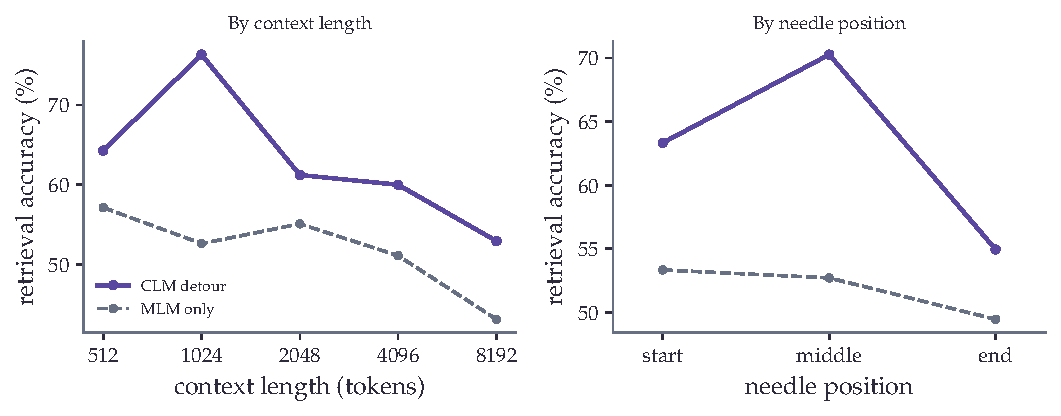
\includegraphics[width=\textwidth]{plots/chapter5/needle.pdf}
  \caption{Needle-in-a-haystack retrieval in French, binary accuracy of a frozen-encoder
  probe. The CLM detour stays above the MLM-only model at every context length (left) and
  at every needle position (right), with the largest margin at mid-document.}
  \label{fig:needle}
\end{figure}

\begin{reviewread}
Long-context encoding is critical in biomedical NLP, where clinical documents routinely span thousands of tokens and key information (diagnoses, coding labels) can appear anywhere in the document. We design a synthetic needle-in-a-haystack task in French to evaluate long-context retrieval without entity-type confounds.
\end{reviewread}

\paragraph{Protocol.} A medical fact (the ``needle'') is inserted into a clinical document (the ``haystack'') at a controlled position, and the model must determine whether a given query fact is present (binary classification). Negative examples use the same template with different slot values, so the task requires precise retrieval rather than shallow pattern matching. We define 8 French medical fact templates covering drugs, vital signs, lab results, diagnoses, procedures, allergies, treatment duration, and symptoms. Each template has 2--4 slots filled from small lexicons:

\begin{itemize}
  \item \textit{Le patient a re\c{c}u 200\,mg de morphine par voie intraveineuse.}\\
        \textbf{Distractor:} \textit{Le patient a re\c{c}u 500\,mg de tramadol par voie orale.}
  \item \textit{La tension art\'erielle mesur\'ee \'etait de 160/90\,mmHg.}
  \item \textit{Le diagnostic retenu est cirrhose h\'epatique de stade~III.}
  \item \textit{Le patient rapporte une dyspn\'ee \'evoluant depuis une semaine.}
\end{itemize}

\begin{reviewread}
We generate 1,500 balanced positive/negative pairs across 5 lengths (512--8,192 tokens) and 3 positions (start, middle, end), split 70/15/15 for train/validation/test. We freeze each encoder and train a 2-layer MLP probe (Dropout $\to$ Linear $\to$ GELU $\to$ Dropout $\to$ Linear) on CLS representations for 3 epochs (lr $= 2 \times 10^{-5}$, batch size 4, AdamW), selecting the best checkpoint by validation accuracy.
\end{reviewread}

\paragraph{Results.} CLM outperforms MLM at every context length and position (\Cref{fig:needle}; +10.7pp overall: 62.2\% vs 51.6\%). MLM accuracy degrades monotonically with document length (57\% at 512 tokens to 43\% at 8,192), while CLM degrades more slowly and remains above MLM throughout. The CLM advantage is largest at mid-document positions, where the inserted fact is farthest from both sequence boundaries. This is consistent with the downstream pattern: the French tasks with the largest CLM gains (FrACCO, CANTEMIST) use sequence lengths of 4,096 tokens during fine-tuning.


\section{Analysis: Why Does the CLM Detour Work?}
\label{sec:analysis}

\subsection{CKA Methodology}
\label{sec:cka_method}

We measure representational similarity with linear Centered Kernel Alignment~\citep{kornblith2019similarity}. Given two representation matrices $X \in \mathbb{R}^{n \times p}$ and $Y \in \mathbb{R}^{n \times q}$ (one per model, $n$ samples, mean-pooled over tokens), we center each column, compute Gram matrices $K = XX^\top$ and $L = YY^\top$, and define:
\[
\text{CKA}(X, Y) = \frac{\text{tr}(KL)}{\sqrt{\text{tr}(K^2)\,\text{tr}(L^2)}}
\]
We report divergence $d = 1 - \text{CKA}$, so higher values indicate greater representational difference. CKA equals 1 when representations are identical up to invertible linear transformation, 0 when there is no linear relationship. All computations use float64 arithmetic. For French we use 500 held-out texts from DiaMED and FrACCO; for English, PubMed abstracts. Results are averaged over 3 seeds.

\subsection{The CLM Imprint Persists in Low Layers}
\label{sec:persistence}

\begin{figure}[t]
  \centering
  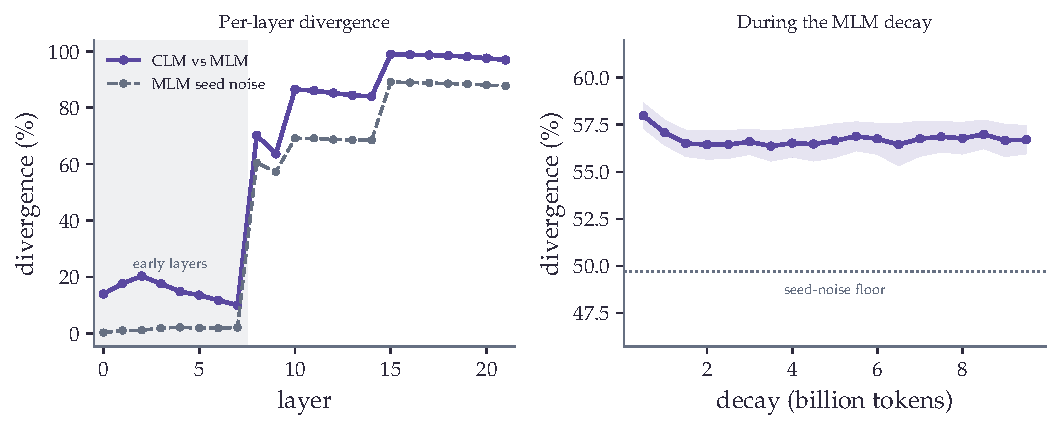
\includegraphics[width=\textwidth]{plots/chapter5/cka_mechanism.pdf}
  \caption{Where the detour leaves its mark, measured by representational divergence
  ($1-\text{CKA}$, held-out clinical text, three seeds). Left: per layer, the CLM-vs-MLM
  pair against a same-objective seed-noise control; the early layers diverge several times
  more than the noise floor. Right: during the MLM decay the divergence plateaus well above
  the seed-noise floor, so decaying back to masked training does not return the model to an
  MLM-like state.}
  \label{fig:cka-mechanism}
\end{figure}

\begin{reviewread}
Comparing layer-by-layer CKA between CLM-detour and MLM-only models (\Cref{fig:cka-mechanism}), the CLM phase modifies low-layer representations in a way that subsequent MLM training does not undo, even when the decay budget matches the CLM phase. CKA divergence reaches approximately 56.5\% after 1.5B tokens of MLM decay and remains stable, with only 0.6pp variation over 8B additional tokens.
\end{reviewread}

To isolate where CLM differs from MLM \emph{specifically} rather than just from training noise, we normalize each layer's CLM-MLM divergence by a seed-noise control (two MLM models trained with different random seeds on identical data):
\[
r_\ell = \frac{1 - \text{CKA}(\text{CLM}_\ell,\; \text{MLM}^{s_1}_\ell)}{1 - \text{CKA}(\text{MLM}^{s_2}_\ell,\; \text{MLM}^{s_1}_\ell)}
\]
A ratio of 1 means no CLM-specific effect. Low layers (0--7) show ratios of 5--44$\times$: CLM changes them far more than random seed variation does. Mid and deep layers are near 1$\times$: both objectives modify them similarly, so CKA cannot distinguish CLM from MLM there.

\subsection{Causal Evidence: Freeze Interventions}
\label{sec:freeze-results}

\begin{figure}[t]
  \centering
  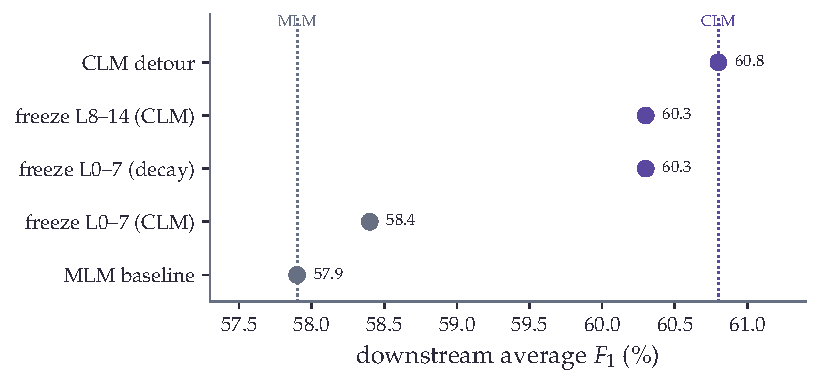
\includegraphics[width=0.8\textwidth]{plots/chapter5/freeze.pdf}
  \caption{Freeze interventions (French Base, 8 tasks, 9 seeds). Freezing the low
  layers during the CLM phase drops the model back onto the MLM baseline, while
  freezing the mid layers, or freezing the low layers during the decay, keeps the
  full gain: the low layers are necessary during the causal phase, the mid layers
  are not.}
  \label{fig:freeze}
\end{figure}

\begin{reviewread}
Do these low-layer changes actually drive the downstream improvement? A freeze experiment holds a group of layers fixed during one phase of training, so that the rest of the model still trains normally around it. If the benefit depends on a layer group being modified during a given phase, freezing that group in that phase should remove the benefit. We run three such experiments on the 22-layer French Base model, where the CLM-MLM gap is largest (+2.9pp):
\end{reviewread}

\begin{itemize}
    \item \textbf{Experiment~1} (low freeze, CLM phase): Layers 0--7 frozen during CLM, then normal decay. Tests whether low-layer modification during CLM is necessary.
    \item \textbf{Experiment~2} (low freeze, decay phase): Normal CLM, then layers 0--7 frozen during decay. Tests whether low-layer CLM changes persist without further updates.
    \item \textbf{Experiment~3} (mid freeze, CLM phase): Layers 8--14 frozen during CLM, then normal decay. Together with Experiment~1, tests selectivity: if freezing low layers eliminates the benefit while freezing mid layers preserves it, this constitutes a double dissociation.
\end{itemize}

\begin{reviewread}
The three conditions are summarized in \Cref{fig:freeze} and \Cref{tab:freeze}.
\end{reviewread}

\begin{table}[t]
\centering
\small
\begin{tabular}{lcc}
\toprule
\textbf{Condition} & \textbf{Avg $F_1$} & $\boldsymbol{\Delta}$ \textbf{vs MLM} \\
\midrule
\rowcolor{ThesisTableSep} \multicolumn{3}{c}{\rule{0pt}{9pt}\textbf{References}} \\[1pt]
MLM baseline & 57.9 & --- \\
CLM detour & \bfseries 60.8 & +2.9 \\
\midrule
\rowcolor{ThesisTableSep} \multicolumn{3}{c}{\rule{0pt}{9pt}\textbf{Freeze interventions}} \\[1pt]
Freeze L0--7 (CLM phase) & 58.4 & +0.5 \\
Freeze L8--14 (CLM phase) & 60.3 & +2.4 \\
Freeze L0--7 (decay phase) & 60.3 & +2.4 \\
\bottomrule
\end{tabular}
\caption{\textbf{Freeze intervention results} (French Base, 8 tasks, 9 seeds). Freezing low layers during CLM eliminates the benefit ($p=0.36$ vs MLM baseline). Freezing mid layers preserves it. Freezing low layers during decay has negligible effect.}
\label{tab:freeze}
\end{table}

\begin{reviewread}
Freezing low layers (0--7) during CLM drops $F_1$ from 60.8\% to 58.4\%. We cannot reject the null hypothesis that the resulting model matches the MLM baseline ($p = 0.36$, paired bootstrap across 8 tasks $\times$ 9 seeds). Freezing mid layers (8--14) during CLM preserves the full benefit (60.3\%). Together, these two experiments establish a double dissociation: low layers are necessary and mid layers are not. Freezing low layers during decay has negligible effect ($-$0.5pp, 60.3\%), confirming that MLM decay preserves the CLM imprint in low layers.
\end{reviewread}

\subsection{Non-Localizability}

\begin{reviewread}
The freeze experiments show that low layers are necessary \emph{during training}. We now ask whether the resulting benefit can be localized \emph{after training}, by copying full parameter blocks from the CLM model into the MLM model.
\end{reviewread}

\begin{table}[t]
\centering
\small
\begin{tabular}{lccc}
\toprule
\textbf{Transplant} & \textbf{$F_1$ (\%)} & $\boldsymbol{\Delta}$ & \textbf{Recovery} \\
\midrule
\rowcolor{ThesisTableSep} \multicolumn{4}{c}{\rule{0pt}{9pt}\textbf{References}} \\[1pt]
MLM baseline & 32.8 & --- & 0\% \\
CLM detour & 39.9 & +7.1 & 100\% \\
\midrule
\rowcolor{ThesisTableSep} \multicolumn{4}{c}{\rule{0pt}{9pt}\textbf{Layer group transplants}} \\[1pt]
Low (0--7) & 31.9 & $-$0.9 & $-$12\% \\
Mid (8--14) & 35.3 & +2.5 & +35\% \\
Late (15--21) & 32.4 & $-$0.4 & $-$6\% \\
\bottomrule
\end{tabular}
\caption{\textbf{Layer transplantation} on DiaMED (3 seeds, linear probing). All transplants recover at most 35\% of the 7.1pp gap.}
\label{tab:transplant}
\end{table}

\begin{reviewread}
No transplant recovers more than 35\% of the gap (\Cref{tab:transplant}). Low and late layer transplants hurt performance. Inserting CLM low layers into an MLM model creates a mismatch with the mid and deep layers that co-adapted under MLM, yielding representations worse than either pure model.
\end{reviewread}

\begin{reviewread}
Component-level transplants (\Cref{tab:transplant-comp}) confirm the same pattern. Replacing all attention modules from CLM into MLM recovers only 15\% of the gap; replacing all MLP blocks recovers 35\%. No single component type captures the full benefit.
\end{reviewread}

\begin{table}[t]
\centering
\small
\begin{tabular}{lccc}
\toprule
\textbf{Transplant} & \textbf{$F_1$ (\%)} & $\boldsymbol{\Delta}$ & \textbf{Recovery} \\
\midrule
All attention & 33.9 & +1.1 & +15\% \\
All MLP & 35.3 & +2.5 & +35\% \\
\bottomrule
\end{tabular}
\caption{\textbf{Component-level transplants} on DiaMED (3 seeds, linear probing). Neither attention nor MLP modules alone recover the full gap.}
\label{tab:transplant-comp}
\end{table}

\begin{reviewread}
Unlike freeze interventions, which act during training, transplants replace already-trained weights and cannot reconstruct the cross-layer co-adaptation that developed during CLM. The freeze experiments show low layers are necessary during training; the transplant experiments show the resulting benefit cannot be isolated post hoc.
\end{reviewread}

\subsection{Scaling and Architectural Asymmetry}
\label{sec:asymmetry}

\begin{table}[t]
\centering
\small
\begin{tabular}{llcc}
\toprule
\textbf{Model} & \textbf{Params} & \textbf{Div.} & \textbf{CI} \\
\midrule
\rowcolor{ThesisTableSep} \multicolumn{4}{c}{\rule{0pt}{9pt}\textbf{Encoders (MLM$\to$CLM$\to$MLM)}} \\[1pt]
ModernCamemBERT Base & 150M & 56.5\% & $\pm$0.7\% \\
ModernCamemBERT Large & 350M & 67.2\% & $\pm$0.3\% \\
\midrule
\rowcolor{ThesisTableSep} \multicolumn{4}{c}{\rule{0pt}{9pt}\textbf{Decoder (CLM$\to$MLM$\to$CLM)}} \\[1pt]
Gemma-3 & 270M & 26.3\% & $\pm$1.0\% \\
\bottomrule
\end{tabular}
\caption{\textbf{CKA divergence scales with model size and is asymmetric.} The encoder-decoder comparison uses different model families (see text).}
\label{tab:asymmetry}
\end{table}

\begin{reviewread}
The CLM imprint increases with model capacity (\Cref{tab:asymmetry}): Large (350M) reaches 67.2\% $\pm$ 0.3\% divergence versus 56.5\% $\pm$ 0.7\% for Base (150M). Testing the reverse on Gemma-3 (270M decoder), MLM-then-CLM retains only 26.3\% $\pm$ 1.0\% divergence versus 67.2\% for an encoder of similar scale. One explanation is the density of the decay signal: MLM decay at 15\% masking provides weak erasure, while CLM decay at 100\% provides strong erasure. This comparison is exploratory: it is confounded by model family and language, and a controlled comparison using encoder and decoder variants of the same family would be needed to confirm the asymmetry.
\end{reviewread}


\section{Limitations}

\begin{reviewread}
Our freeze interventions use French Base models only. The CKA patterns that motivate them (low-layer divergence well above seed noise) are consistent across French Base, French Large, and English Base, but replication of the freeze interventions on English and Large models would strengthen the causal claim. The encoder-decoder asymmetry comparison is confounded by model family. The position trade-off at 2048+ tokens means that the approach may not be suitable for tasks requiring very long context, such as full discharge summary coding.
\end{reviewread}


\section*{Conclusion}

\begin{reviewread}
Training an encoder like a decoder, then converting it back, produces stronger representations than training with MLM alone. The CLM detour reshapes low transformer layers in ways that subsequent MLM decay does not undo: a lasting imprint that scales with model capacity and produces consistent downstream gains across 8 French and 11 English biomedical tasks.
\end{reviewread}

\begin{reviewread}
For biomedical encoder pretraining, the CLM detour improves results at no extra cost, using the same data and the same compute budget as MLM-only pretraining. MLM decay of roughly 10\% of the detour length suffices, and the effect is strongest when the domain gap between pretraining and target data is large.
\end{reviewread}

\vspace{2em}

\begin{reviewread}
Parts~1 and 2 of this thesis have focused on data and pretraining: how to collect biomedical text, how to filter it, and how to train encoder models on it. But a pretrained model is only useful if it can be deployed on real tasks. In the next part, we turn to adaptation: how to extract clinical information when labeled data is scarce, labels number in the thousands, and the only available text is public.
\end{reviewread}
